% G2-3 Pertumbuhan pohon level-wise dan leaf-wise.
% Sumber: diadaptasi dari lightgbmfeatures (bukan ke2017).
% Dasar: gambar v2.9 di chapters/bab2-tinjauan-pustaka.tex, disimpan sebagai
% file baru tanpa mengubah yang lama.
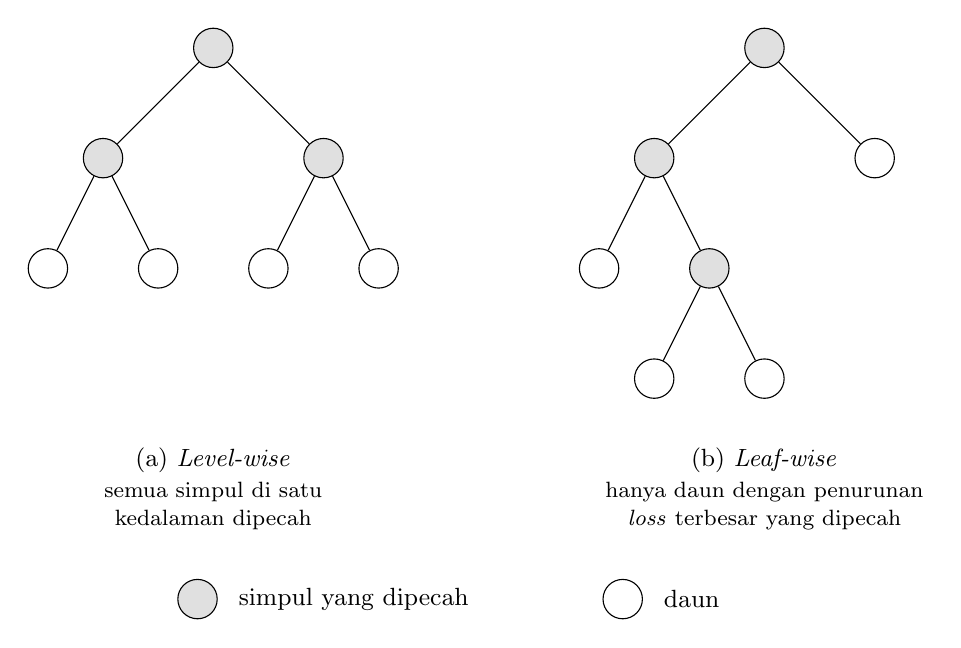
\begin{tikzpicture}[x=1mm,y=-1mm,font=\small,
    simpul/.style={draw,circle,inner sep=0pt,minimum size=5mm},
    pecah/.style={draw,circle,fill=black!12,inner sep=0pt,minimum size=5mm}]

  % --- panel kiri: level-wise ---
  \begin{scope}
    \node[pecah]  (a) at (28,0)  {};
    \node[pecah]  (b) at (14,14) {};
    \node[pecah]  (c) at (42,14) {};
    \node[simpul] (d) at (7,28)  {};
    \node[simpul] (e) at (21,28) {};
    \node[simpul] (f) at (35,28) {};
    \node[simpul] (g) at (49,28) {};
    \draw (a) -- (b) (a) -- (c) (b) -- (d) (b) -- (e) (c) -- (f) (c) -- (g);
    \node[align=center] at (28,56)
      {(a) \textit{Level-wise}\\
       \footnotesize semua simpul di satu\\[-1pt]
       \footnotesize kedalaman dipecah};
  \end{scope}

  % --- panel kanan: leaf-wise ---
  \begin{scope}[xshift=70mm]
    \node[pecah]  (a2) at (28,0)  {};
    \node[pecah]  (b2) at (14,14) {};
    \node[simpul] (c2) at (42,14) {};
    \node[simpul] (d2) at (7,28)  {};
    \node[pecah]  (e2) at (21,28) {};
    \node[simpul] (f2) at (14,42) {};
    \node[simpul] (g2) at (28,42) {};
    \draw (a2) -- (b2) (a2) -- (c2) (b2) -- (d2) (b2) -- (e2)
          (e2) -- (f2) (e2) -- (g2);
    \node[align=center] at (28,56)
      {(b) \textit{Leaf-wise}\\
       \footnotesize hanya daun dengan penurunan\\[-1pt]
       \footnotesize \textit{loss} terbesar yang dipecah};
  \end{scope}

  % --- legenda ---
  \node[pecah] at (26,70) {};
  \node[anchor=west] at (30,70) {simpul yang dipecah};
  \node[simpul] at (80,70) {};
  \node[anchor=west] at (84,70) {daun};
\end{tikzpicture}
